\documentclass[10pt,twocolumn,letterpaper]{article}

% ------------------------------------------------------------------
% Packages
% ------------------------------------------------------------------
\usepackage[utf8]{inputenc}
\usepackage[T1]{fontenc}
\usepackage{mathptmx}                 % Times-like text and math
\usepackage[margin=0.75in,columnsep=0.25in]{geometry}
\usepackage{amsmath,amssymb}
\usepackage{graphicx}
\usepackage{booktabs}
\usepackage{multirow}
\usepackage[font=small,labelfont=bf,skip=4pt]{caption}
\usepackage{subcaption}
\usepackage{tikz}
\usetikzlibrary{arrows.meta,positioning,fit,calc}
\usepackage{enumitem}
\usepackage{titlesec}
\usepackage{xcolor}
\usepackage{microtype}
\usepackage[colorlinks=true,urlcolor=blue!60!black,linkcolor=black,citecolor=black]{hyperref}
\usepackage{balance}

\setlist{nosep,leftmargin=*}
\titleformat{\section}{\normalfont\large\bfseries}{\thesection.}{0.5em}{}
\titleformat{\subsection}{\normalfont\normalsize\bfseries}{\thesubsection}{0.5em}{}
\titlespacing*{\section}{0pt}{8pt}{3pt}
\titlespacing*{\subsection}{0pt}{6pt}{2pt}
\setlength{\textfloatsep}{8pt plus 2pt minus 2pt}
\setlength{\floatsep}{6pt plus 2pt minus 2pt}

\newcommand{\eps}{\varepsilon}

% ------------------------------------------------------------------
\title{\vspace{-1.2em}\textbf{Reinforcement Learning and DQN on Gymnasium Environments}}
\author{Tamya Chilca\~{n}an \qquad Adriana Espinoza\\[2pt]
\small Code and results: \url{https://github.com/adrianasofiaespinoza/proyecto_agentesinteligentes}}
\date{}

\begin{document}
\maketitle

% ==================================================================
\begin{abstract}
We compare tabular Q-learning and Deep Q-Networks (DQN) on Gymnasium control tasks under a shared, reproducible protocol (three training seeds, identical step budgets, greedy evaluation on fixed seeds). On CartPole-v1 with a 300k-step budget, tabular Q-learning with 10 bins per dimension reached a final return of $493.9\pm5.1$ (mean $\pm$ std across seeds, 3/3 seeds solved), whereas DQN reached $369.5\pm184.5$ (2/3 solved): two DQN seeds were perfect, but one collapsed from 500 to 108.5 after having solved the task. On LunarLander-v3, DQN solved the task in all seeds ($250.2\pm9.3$). Ablations show that the replay buffer is the most critical component (0/3 seeds solved without it, with a $+48$ overestimation of the initial-state value), while the target network trades speed for stability, a trend confirmed by varying its update period from 100 to 5000 steps. Double DQN improved stability and speed on CartPole ($473.8\pm37.1$; threshold reached at 120k--130k steps vs.\ 170k--200k), where vanilla DQN overestimated the value of the initial state, but brought no significant change on LunarLander, where overestimation was small. We relate these findings to locality of tabular updates, catastrophic forgetting and maximisation bias.
\end{abstract}

% ==================================================================
\section{Introduction}

Value-based reinforcement learning (RL) estimates the action-value function $Q(s,a)$ and acts greedily with respect to it. Tabular Q-learning~\cite{watkins1992,sutton2018} stores one value per state--action pair and converges under classical conditions, but it requires a small, discrete state space. DQN~\cite{mnih2015} replaces the table by a neural network, which allows generalisation to large or continuous state spaces at the cost of stability: bootstrapped targets, correlated samples and function approximation can make training oscillate or diverge.

This project asks three questions: (i) on a problem small enough for both methods, which one learns faster and more reliably, and why? (ii) which DQN components and hyperparameters matter on a harder task? (iii) does Double DQN~\cite{vanhasselt2016}, which targets the maximisation bias of DQN, actually help in our setting? Our contributions are:
\begin{itemize}
  \item \textbf{Tier 1:} a fair comparison of Q-learning and DQN on CartPole-v1 with equal step budgets, including a discretisation study for the tabular agent.
  \item \textbf{Tier 2:} DQN on LunarLander-v3 with a hyperparameter study (learning rate and target-network update period) and ablations of the target network and the replay buffer.
  \item \textbf{Tier 3:} Double DQN against vanilla DQN on both environments, with a direct measurement of value overestimation.
  \item An analysis of why locomotion and pixel-based tasks are unsuitable for these methods.
\end{itemize}

% ==================================================================
\section{Pertinence Analysis}
\label{sec:pertinence}

Tabular methods need a state space that is small after discretisation; DQN needs a discrete action space, because it outputs one value per action and acts with $\arg\max_a Q(s,a)$. Table~\ref{tab:envs} summarises the two Gymnasium~\cite{towers2024} environments used.

\textbf{CartPole-v1} has 4 continuous observations (cart position and velocity, pole angle and angular velocity) and 2 actions. With $b$ bins per dimension the table has $b^4$ states: 1{,}296 for $b=6$, 10{,}000 for $b=10$ and 160{,}000 for $b=20$, i.e.\ at most $3.2\times10^5$ entries. A few hundred thousand environment steps can visit the relevant part of this table, so CartPole suits \emph{both} methods and allows a direct comparison.

\textbf{LunarLander-v3} has 8 observations (6 continuous, 2 binary leg contacts) and 4 discrete actions. Even 10 bins on the six continuous dimensions give $10^6\times 2^2=4\times10^6$ states, and the coarse grid would destroy the fine control needed for a soft landing. The action space, however, is discrete and small, which makes the task a natural fit for DQN and a poor fit for a table.

\begin{table}[t]
\centering
\caption{Environments used (Gymnasium 1.x).}
\label{tab:envs}
\small
\setlength{\tabcolsep}{4pt}
\begin{tabular}{@{}lccccc@{}}
\toprule
Environment & Obs. & Actions & Threshold & Budget & Tier \\
\midrule
CartPole-v1    & 4 cont.  & 2 disc. & $\ge 475$ & 300k & 1, 3 \\
LunarLander-v3 & 8 (6+2)  & 4 disc. & $\ge 200$ & 500k & 2, 3 \\
\bottomrule
\end{tabular}
\vspace{2pt}

\footnotesize Threshold: mean return over 100 greedy episodes. Budget: environment steps per seed.
\end{table}

% ==================================================================
\section{Methods}

\subsection{Tabular Q-learning with state discretisation}
Each observation dimension $i$ is clipped implicitly to $[\ell_i,u_i]$ and split into $b$ equal-width bins, mapping the continuous state to a tuple of four indices. The table is initialised to zero and updated after every transition $(s,a,r,s')$:
\begin{equation}
Q(s,a) \leftarrow Q(s,a) + \alpha\big[\,r + \gamma\,(1-d)\max_{a'} Q(s',a') - Q(s,a)\big],
\label{eq:qlearning}
\end{equation}
where $d=1$ only if the episode \emph{terminated} (the pole fell or the cart left the track). Actions are $\eps$-greedy with random tie-breaking, so that unvisited states (all zeros) are explored uniformly.

\subsection{Deep Q-Network}
DQN approximates $Q(s,\cdot)$ with a multilayer perceptron $Q_\theta$ that outputs one value per action (Fig.~\ref{fig:dqn}). Transitions are stored in a circular replay buffer~\cite{lin1992} and minibatches $\mathcal{B}$ are sampled uniformly, which breaks the temporal correlation of consecutive samples. The target uses a frozen copy $Q_{\theta^-}$ of the network, synchronised every $C$ steps:
\begin{equation}
y = r + \gamma\,(1-d)\,\max_{a'} Q_{\theta^-}(s',a'),
\label{eq:dqn}
\end{equation}
and $\theta$ minimises the Huber loss $\frac{1}{|\mathcal{B}|}\sum \mathcal{L}_\delta\big(y - Q_\theta(s,a)\big)$ with Adam, as in~\cite{mnih2015}; gradients are clipped to norm 10. Exploration is $\eps$-greedy with $\eps$ decayed linearly from 1.0 to 0.05.

A subtle but important detail concerns episode ends. Gymnasium distinguishes \emph{termination} (a true terminal state) from \emph{truncation} (the time limit: 500 steps in CartPole, 1000 in LunarLander). We set $d=1$ only on termination; on truncation the next state still has future value, so the target keeps bootstrapping. Treating truncation as terminal would teach the agent that reaching the time limit is a failure.

\begin{figure}[t]
\centering
\resizebox{\columnwidth}{!}{%
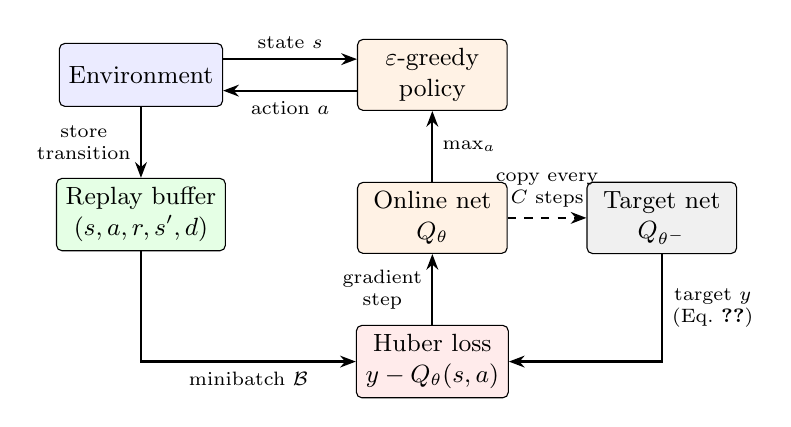
\begin{tikzpicture}[
  box/.style={draw, rounded corners=2pt, minimum height=8mm, minimum width=19mm, align=center, font=\small, fill=#1},
  box/.default=white,
  arr/.style={-{Stealth[length=2mm]}, thick},
  lbl/.style={font=\scriptsize, align=center}]
\node[box=blue!8] (env) {Environment};
\node[box=orange!10, right=17mm of env] (agent) {$\eps$-greedy\\policy};
\node[box=green!10, below=9mm of env] (buf) {Replay buffer\\$(s,a,r,s',d)$};
\node[box=orange!10, below=9mm of agent] (online) {Online net\\$Q_\theta$};
\node[box=gray!12, right=10mm of online] (target) {Target net\\$Q_{\theta^-}$};
\node[box=red!8, below=9mm of online] (loss) {Huber loss\\$y - Q_\theta(s,a)$};
\draw[arr] ([yshift=-2mm]agent.west) -- node[below,lbl]{action $a$} ([yshift=-2mm]env.east);
\draw[arr] (env.south) -- node[left,lbl]{store\\transition} (buf.north);
\draw[arr] (buf.south) |- node[below,pos=0.75,lbl]{minibatch $\mathcal{B}$} (loss.west);
\draw[arr] (online) -- node[right,lbl]{$\max_a$} (agent);
\draw[arr] (target.south) |- node[right,pos=0.25,lbl]{target $y$\\(Eq.~\ref{eq:dqn})} (loss.east);
\draw[arr] (loss.north) -- node[left,lbl]{gradient\\step} (online.south);
\draw[arr, dashed] (online.east) -- node[above,lbl]{copy every\\$C$ steps} (target.west);
\draw[arr] ([yshift=2mm]env.east) -- node[above,lbl]{state $s$} ([yshift=2mm]agent.west);
\end{tikzpicture}}
\caption{DQN training loop as implemented. Double DQN only changes how the target $y$ is computed (Eq.~\ref{eq:ddqn}).}
\label{fig:dqn}
\end{figure}

\subsection{Double DQN}
The $\max$ in Eq.~\eqref{eq:dqn} both \emph{selects} and \emph{evaluates} the next action with the same noisy estimates, which biases the target upwards~\cite{thrun1993,vanhasselt2016}. Double DQN decouples the two steps, using the online network to select and the target network to evaluate:
\begin{equation}
y^{\text{DDQN}} = r + \gamma\,(1-d)\,Q_{\theta^-}\!\big(s',\,\arg\max_{a'} Q_\theta(s',a')\big).
\label{eq:ddqn}
\end{equation}
Everything else (network, buffer, schedule, hyperparameters) is identical to vanilla DQN, so any difference is attributable to Eq.~\eqref{eq:ddqn}.

\subsection{Ablation variants}
\textbf{No target network:} $Q_{\theta^-}\equiv Q_\theta$, so the target moves with every gradient step. \textbf{No replay buffer:} the buffer keeps only the most recent 128 transitions and each update uses all of them in temporal order; with one update every 4 steps, each transition is reused about 32 times in a row and samples remain strongly correlated.

% ==================================================================
\section{Experimental Settings}

\textbf{Protocol.} Every configuration was trained with seeds 42, 123 and 456, which fix the environment, NumPy and PyTorch generators. Every 10{,}000 steps the agent was evaluated greedily ($\eps=0$) on 10 episodes with fixed seeds 10000--10009; these points form the learning curves, which are plotted against \emph{environment steps}, not episodes, so that both methods share the same x-axis. After training, the final policy was evaluated on 100 greedy episodes with seeds 20000--20099, disjoint from the curve seeds. We report the mean of the per-seed means $\pm$ their standard deviation across seeds, the number of seeds whose final mean reaches the threshold, the first step at which a 10-episode evaluation reached the threshold (``steps to threshold''), and training wall-clock time excluding evaluation. The value of the best intermediate checkpoint is logged but reported separately, since checkpoint selection is itself a design choice.

\textbf{Overestimation probe.} At every evaluation we log $\max_a Q_\theta(s_0,a)$, the agent's own estimate of the initial state value, together with the discounted return actually obtained from $s_0$. A dashed curve above the solid one indicates overestimation.

\textbf{Hyperparameters} are listed in Table~\ref{tab:hparams}. For DQN on CartPole, an initial configuration (learning rate $5\times10^{-4}$, buffer 50k, batch 64, $C=500$) was run once on seeds 42 and 123 and was clearly unstable (one seed ended at 107). We then compared configurations only on held-out seeds 0 and 1 and kept the one in Table~\ref{tab:hparams}, which ended at 500 on both. The LunarLander configuration was validated with a single run before launching all seeds. The tabular configuration comes from the design study in Section~\ref{sec:tier1}.

\textbf{Hardware and software.} All runs used CPU only, on two laptops: one with 16 logical cores and 16\,GB of RAM (Arch Linux, Python 3.14, PyTorch, Gymnasium 1.x; one thread per process), used for most DQN runs, all LunarLander runs and every reported time; and one with 4 cores and 8\,GB of RAM, used for development, plotting and part of Tier~1. The 24 LunarLander runs shared the CPU, so their wall-clock times (about 40 minutes, against 5.3 for a single run alone) are only comparable with each other.

\begin{table}[t]
\centering
\caption{Hyperparameters. DQN rows apply to vanilla DQN, Double DQN and the ablations unless stated otherwise.}
\label{tab:hparams}
\small
\setlength{\tabcolsep}{3.5pt}
\resizebox{\columnwidth}{!}{%
\begin{tabular}{@{}lcc@{}}
\toprule
\multicolumn{3}{@{}l}{\textbf{Q-learning (CartPole)}} \\
\midrule
Bins per dimension & \multicolumn{2}{c}{10} \\
Bounds $[\ell,u]$ (pos., vel., angle, ang.\ vel.) & \multicolumn{2}{c}{$\pm2.4,\ \pm2.0,\ \pm0.2095,\ \pm2.5$} \\
$\alpha$, $\gamma$ & \multicolumn{2}{c}{0.1, 0.99} \\
$\eps$ schedule & \multicolumn{2}{c}{$1.0\to0.05$ over 150k steps} \\
\midrule
\textbf{DQN} & \textbf{CartPole} & \textbf{LunarLander} \\
\midrule
Network (ReLU MLP) & 128--128 & 256--256 \\
Learning rate (Adam) & $1\times10^{-4}$ & $5\times10^{-4}$ \\
Batch size & 128 & 128 \\
Replay buffer & 100k & 100k \\
Target update period $C$ & 1000 & 1000 \\
Updates per env.\ step & 1 & 1/4 \\
Learning starts & 1k & 10k \\
$\eps$ schedule ($1.0\to0.05$) & first 30k steps & first 100k steps \\
$\gamma$, Huber $\delta$, grad.\ clip & \multicolumn{2}{c}{0.99, 1, 10} \\
\bottomrule
\end{tabular}}
\end{table}

% ==================================================================
\section{Results}

\subsection{Tier 1: Q-learning versus DQN on CartPole-v1}
\label{sec:tier1}

\textbf{Tabular design study.} Table~\ref{tab:qdesign} reports the tuning of the tabular agent (200k steps, 3 seeds, 100 evaluation episodes). With a fixed $\eps=0.1$, $\alpha=0.5$ and wide velocity bounds ($\pm3.0$, $\pm3.5$), 10 bins worked best and 20 bins worst: with $20^4=160{,}000$ states, each state is visited too rarely in 200k steps, whereas 6 bins are too coarse to separate states that need different actions. A decaying $\eps$ alone did not raise the mean, but a smaller step size ($\alpha=0.1$) did, and narrowing the velocity bounds to the region actually visited (``bounds A'') gave the largest gain, because it spends the 10 bins where the states are instead of on velocities that never occur. Extending the budget, the mean was 394.9 at 200k, 491.1 at 300k and 444.7 at 400k steps; 300k was chosen.

\begin{table}[t]
\centering
\caption{Tabular Q-learning design study on CartPole (3 seeds, 200k steps unless noted; final mean over 100 greedy episodes). Each row changes one factor with respect to the previous best.}
\label{tab:qdesign}
\small
\setlength{\tabcolsep}{4pt}
\begin{tabular}{@{}llc@{}}
\toprule
Factor & Setting & Mean $\pm$ std (seeds) \\
\midrule
\multirow{3}{*}{Bins ($\eps=0.1$, $\alpha=0.5$)} & 6  & $196.3\pm69.6$ \\
                                          & \textbf{10} & $\mathbf{218.1\pm108.9}$ \\
                                          & 20 & $145.9\pm50.9$ \\
\midrule
Exploration & decaying $\eps$ & $212.7$ \\
\midrule
\multirow{2}{*}{Step size $\alpha$} & 0.3 & $274.4$ \\
                                    & \textbf{0.1} & $\mathbf{297.1\pm133.3}$ \\
\midrule
\multirow{2}{*}{Velocity bounds} & B: $\pm1.5$, $\pm2.0$ & $354.9\pm97.0$ \\
                                 & \textbf{A: $\pm2.0$, $\pm2.5$} & $\mathbf{394.9\pm139.1}$ \\
\midrule
\multirow{2}{*}{Budget (bounds A)} & \textbf{300k} & $\mathbf{491.1\pm5.7}$ (3/3) \\
                                   & 400k & $444.7\pm56.8$ (1/3) \\
\bottomrule
\end{tabular}
\end{table}

\textbf{Comparison.} Table~\ref{tab:tier1} and Fig.~\ref{fig:tier1} compare both methods at 300k steps. The tabular runs in the table were re-executed from the original Q-learning code with the same protocol as DQN, adding only the intermediate evaluations (which use their own generator and do not alter training); seed 123 reproduced the original result exactly (486.84), and the mean (493.9) is within 3 points of the original (491.1). Q-learning ended higher and far more consistently across seeds, and trained about 15 times faster in wall-clock time. In environment steps the gap is smaller: Q-learning improved earlier (it leads between 30k and 190k steps) and reached the threshold at 140k--190k steps, against 170k--200k for DQN. DQN reached 500 in all three seeds around 200k steps, but after 210k one seed (42) collapsed and finished at 108.5, while its best checkpoint still scored 500. Q-learning was not perfectly stable either: its mean curve drops to about 280 at 170k steps and oscillates between 380 and 450 from 240k to 280k steps, recovering at 300k.

\begin{table}[t]
\centering
\caption{Tier 1 and Tier 3 on CartPole-v1 (300k steps, 100 greedy episodes per seed, seeds 20000--20099).}
\label{tab:tier1}
\small
\setlength{\tabcolsep}{3pt}
\resizebox{\columnwidth}{!}{%
\begin{tabular}{@{}lccc@{}}
\toprule
 & Q-learning & DQN & Double DQN \\
\midrule
Final mean $\pm$ std (seeds) & $\mathbf{493.9\pm5.1}$ & $369.5\pm184.5$ & $473.8\pm37.1$ \\
Seeds 42 / 123 / 456 & 499.0 / 486.8 / 495.8 & 108.5 / 500 / 500 & 421.2 / 500 / 500 \\
Seeds solved & \textbf{3/3} & 2/3 & 2/3 \\
Steps to threshold & 140k--190k & 170k--200k & \textbf{120k--130k} \\
Best checkpoint & -- & 500.0 & 500.0 \\
Train time (min) & \textbf{0.5} & 7.4 & 7.2 \\
$\max_a Q(s_0,a)$ at end & -- & 109.5 & 106.0 \\
\bottomrule
\end{tabular}}
\end{table}

\begin{figure}[t]
\centering
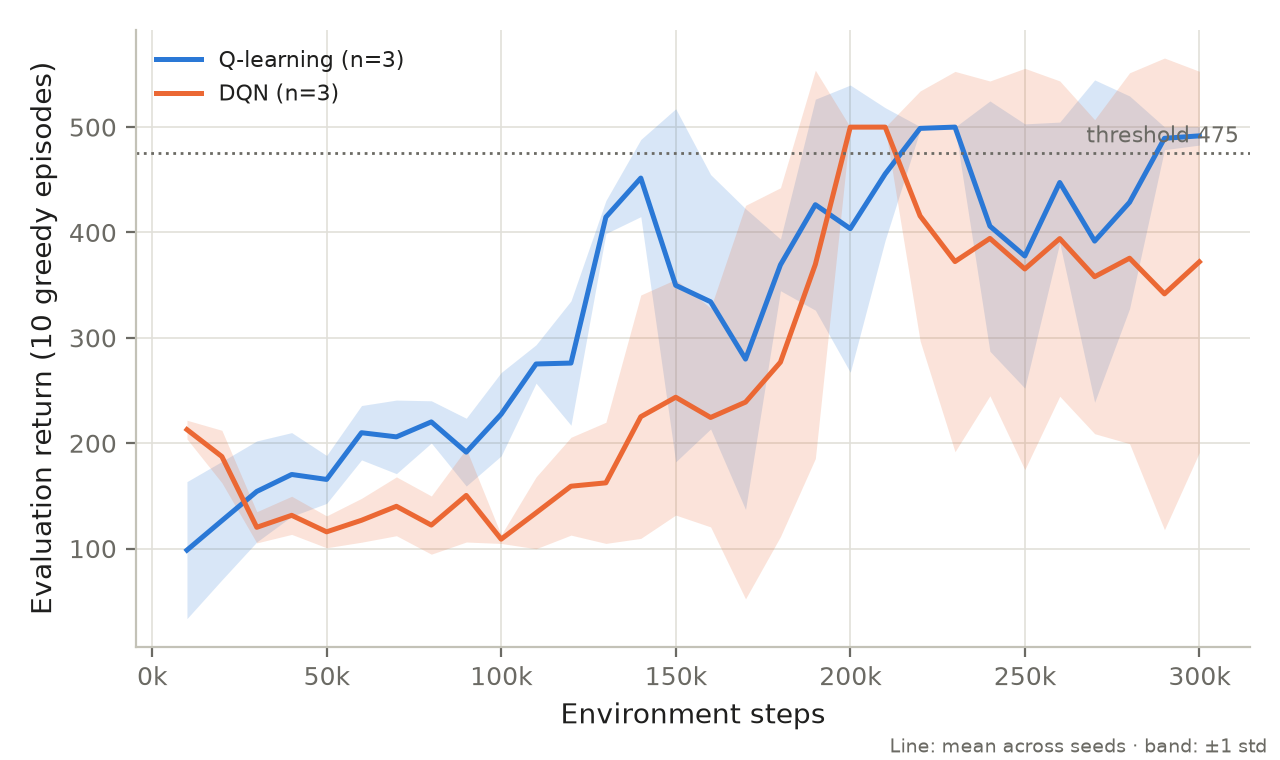
\includegraphics[width=\columnwidth]{figures/tier1_cartpole.png}
\caption{Tier 1: learning curves on CartPole-v1 (mean over 3 seeds, band $\pm1$ std, 10 greedy evaluation episodes every 10k steps).}
\label{fig:tier1}
\end{figure}

\subsection{Tier 2: DQN on LunarLander-v3}

With the default configuration, DQN solved LunarLander in all seeds ($250.2\pm9.3$; Table~\ref{tab:tier2}), reaching the threshold at 190k--270k steps. Fig.~\ref{fig:tier2} shows the ablations and the hyperparameter study.

\textbf{Ablations.} Removing the replay buffer was the most damaging change: no seed solved the task, the curve contains collapses down to about $-580$ (at 30k and 90k steps) and stays below the other variants throughout. It also produced the largest overestimation: the estimated initial value was 82.0 against an actual discounted return of 33.9 (Fig.~\ref{fig:appendix}a). Removing the target network had the opposite profile: the agent learned \emph{faster} (threshold at 70k--110k steps) and its best checkpoint was the best of all runs (261.5), but it ended lower and more variable ($214.5\pm31.1$, 2/3) and showed a short divergence of the value estimate near 450k steps.

\textbf{Learning rate.} The default $5\times10^{-4}$ was the best compromise. A larger rate ($2\times10^{-3}$) learned faster (threshold at 70k--180k) but ended less consistent ($204.7\pm35.8$), and a smaller one ($10^{-4}$) learned slowly (330k--350k) and one seed never solved the task. That seed ended at 1.4: all 100 of its final evaluation episodes reached the 1000-step time limit, with no crash and no completed landing. The agent descends onto the pad but never switches its engines off, so it never collects the $+100$ landing bonus while paying fuel costs (Fig.~\ref{fig:frames}, bottom). This is a known local optimum of LunarLander: the $-100$ crash penalty is learned early, and the action sequence that leads to the landing bonus is rarely explored once $\eps=0.05$.

\textbf{Target update period.} Together with the ablation (period 1), the study yields a monotonic trend (Table~\ref{tab:tier2}): updating more often learns faster but less stably (period 100: threshold as early as 90k steps, one seed ending at 72.7), while updating less often is slower but smoother (period 5000: threshold at 200k--230k in all seeds, $223.7\pm25.2$). The period of 1000 steps gave the best final performance.

\begin{table*}[t]
\centering
\caption{Tier 2: DQN on LunarLander-v3 (500k steps, 3 seeds, 100 greedy episodes per seed). $\Delta Q_0$: estimated minus actual discounted value of the initial state at the end of training. Times are inflated by concurrent execution (Section 4) and only comparable within this table.}
\label{tab:tier2}
\small
\resizebox{\textwidth}{!}{%
\begin{tabular}{@{}llcccccc@{}}
\toprule
 & Variant & Final mean $\pm$ std & Seeds 42 / 123 / 456 & Solved & Steps to threshold & Best ckpt & $\Delta Q_0$ \\
\midrule
Default & DQN ($\text{lr}=5\times10^{-4}$, $C=1000$) & $\mathbf{250.2\pm9.3}$ & 248.3 / 262.4 / 239.9 & \textbf{3/3} & 190k--270k & 249.1 & $0.0$ \\
\midrule
\multirow{2}{*}{Ablation} & No target network & $214.5\pm31.1$ & 235.2 / 237.6 / 170.5 & 2/3 & \textbf{70k--110k} & \textbf{261.5} & $+12.4$ \\
 & No replay buffer & $98.1\pm95.1$ & $-34.8$ / 146.6 / 182.6 & 0/3 & 350k, 460k, not reached & 206.5 & $+48.1$ \\
\midrule
\multirow{2}{*}{Learning rate} & $1\times10^{-4}$ & $153.9\pm108.3$ & 1.4 / 241.5 / 218.9 & 2/3 & 330k, 350k, not reached & 163.9 & $+2.9$ \\
 & $2\times10^{-3}$ & $204.7\pm35.8$ & 236.3 / 154.6 / 223.2 & 2/3 & 70k--180k & 252.2 & $+10.3$ \\
\midrule
\multirow{2}{*}{Target period $C$} & 100 & $193.9\pm85.7$ & 72.7 / 254.5 / 254.3 & 2/3 & 90k--360k & 244.1 & $+1.5$ \\
 & 5000 & $223.7\pm25.2$ & 190.4 / 229.2 / 251.4 & 2/3 & 200k--230k & 239.3 & $-9.8$ \\
\bottomrule
\end{tabular}}
\end{table*}

\begin{figure*}[t]
\centering
\begin{subfigure}{0.33\textwidth}\centering
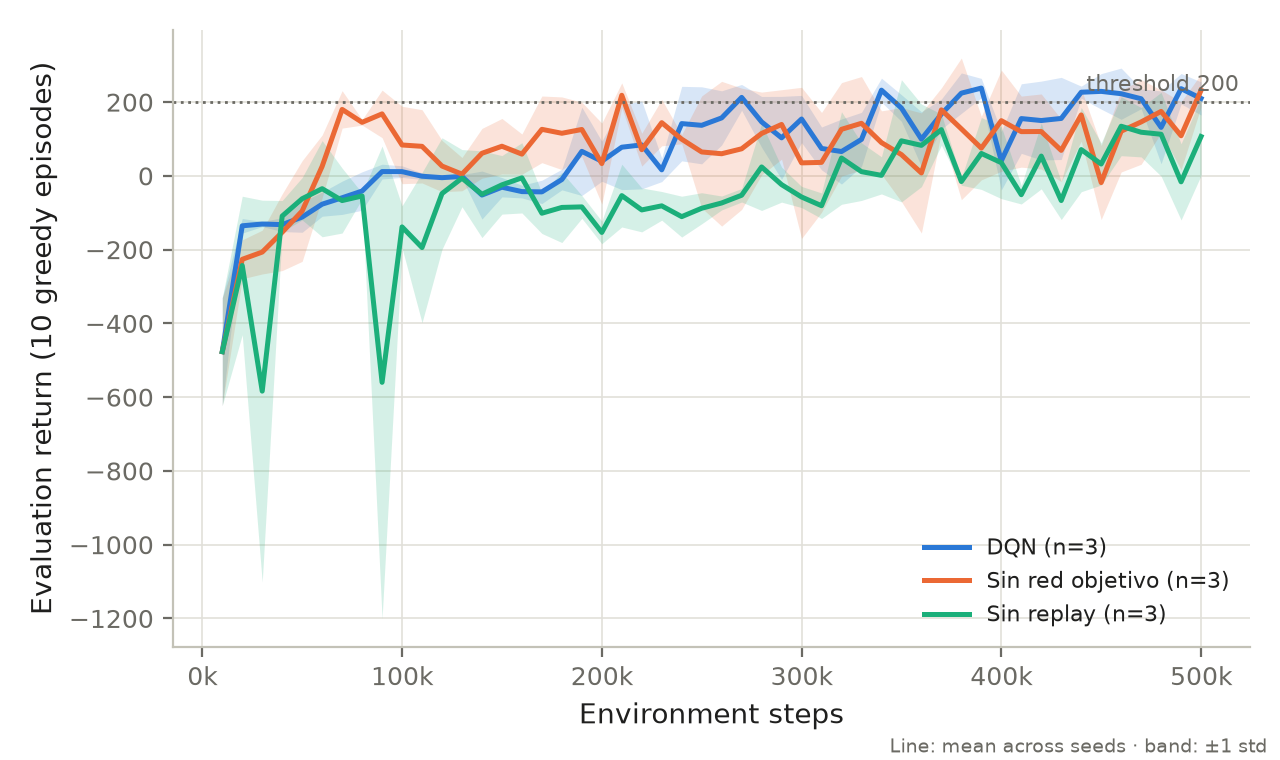
\includegraphics[width=\linewidth]{figures/tier2_ablation.png}
\caption{Ablations.}\end{subfigure}\hfill
\begin{subfigure}{0.33\textwidth}\centering
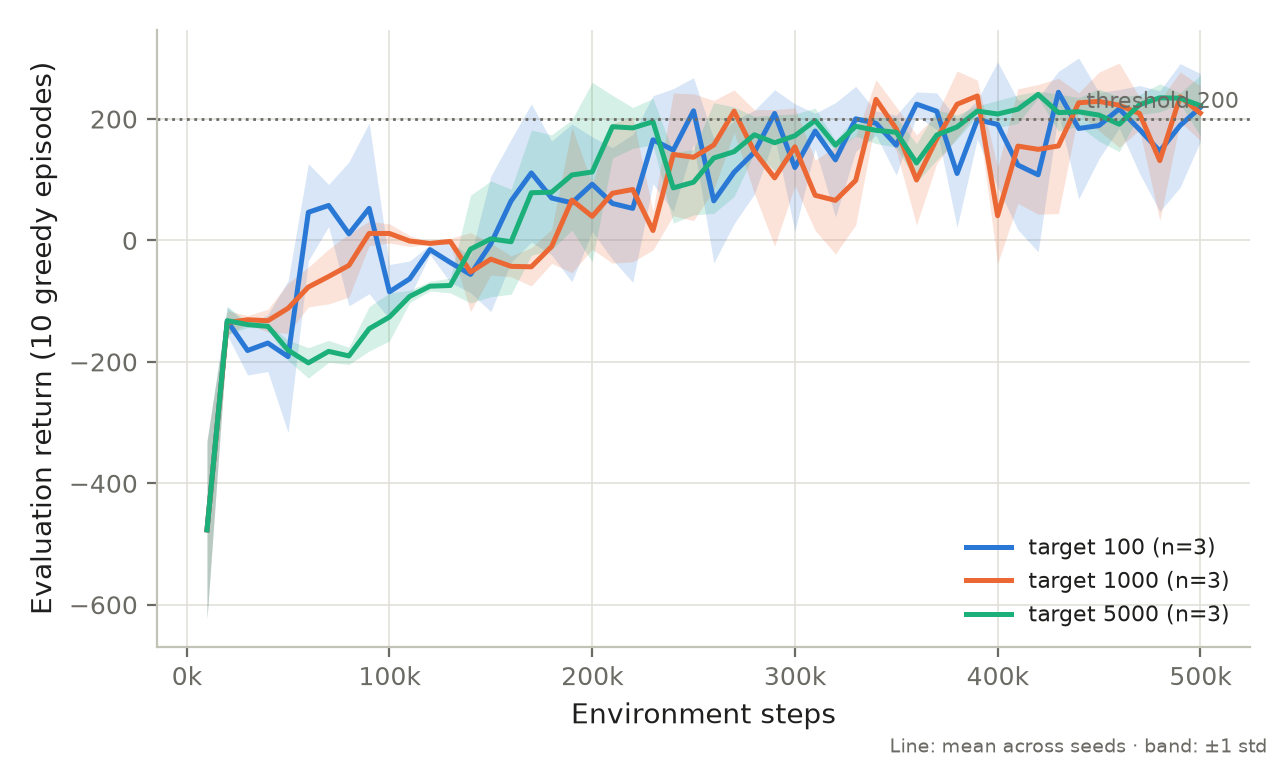
\includegraphics[width=\linewidth]{figures/tier2_target.png}
\caption{Target update period $C$.}\end{subfigure}\hfill
\begin{subfigure}{0.33\textwidth}\centering
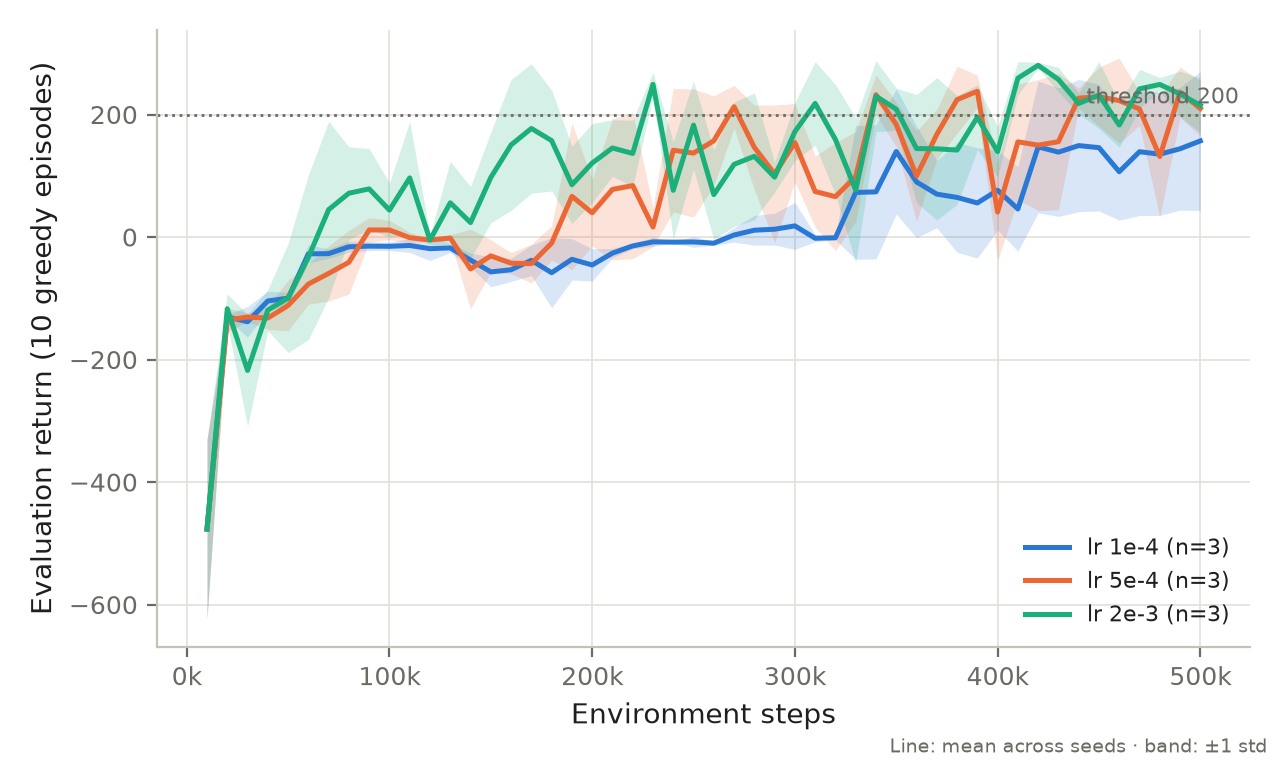
\includegraphics[width=\linewidth]{figures/tier2_lr.png}
\caption{Learning rate.}\end{subfigure}
\caption{Tier 2: evaluation return of DQN on LunarLander-v3 (mean over 3 seeds, band $\pm1$ std; dotted line: threshold 200).}
\label{fig:tier2}
\end{figure*}

\subsection{Tier 3: Double DQN}

Table~\ref{tab:tier3} and Fig.~\ref{fig:tier3} compare vanilla and Double DQN on both environments.

\textbf{CartPole.} Double DQN reduced the spread across seeds from 184.5 to 37.1 and reached the threshold earlier and more uniformly (120k--130k vs.\ 170k--200k steps). The seed that collapsed with DQN (42) ended at 421.2 instead of 108.5; it still misses the threshold, so both methods solve 2/3 seeds. The overestimation probe explains the difference (Fig.~\ref{fig:tier3}b). Because truncation does not stop bootstrapping, the true value of a perfect policy is $1/(1-\gamma)=100$. Both estimates are identical up to about 200k steps; afterwards they keep growing beyond this bound, to 109.5 for DQN and 106.0 for Double DQN. Double DQN therefore reduces, but does not remove, the bias. Early in training both agents \emph{under}estimate $Q(s_0)$, because value propagates backwards through bootstrapping and the target network only changes every 1000 steps.

\textbf{LunarLander.} Here Double DQN gave no significant change in final performance ($240.8\pm28.9$ vs.\ $250.2\pm9.3$; the 10-point gap is far smaller than the 69-point standard deviation across episodes). It improved faster between 80k and 180k steps (about 100 vs.\ 0 in evaluation return) and reached the threshold earlier in two of three seeds (90k and 110k), but the curves converge afterwards. The probe shows why the benefit is limited: both agents overestimated $Q(s_0)$ by about 25 points between 100k and 250k steps, equally, and at the end the estimate matched the actual return for vanilla DQN (71.3 vs.\ 71.3) (Fig.~\ref{fig:appendix}b).

\begin{table}[t]
\centering
\caption{Tier 3: vanilla DQN vs.\ Double DQN (same hyperparameters; 3 seeds, 100 greedy episodes per seed).}
\label{tab:tier3}
\small
\setlength{\tabcolsep}{3pt}
\resizebox{\columnwidth}{!}{%
\begin{tabular}{@{}llcccc@{}}
\toprule
Env. & Method & Final mean & Solved & Steps to thr. & $Q(s_0)$ est./act. \\
\midrule
\multirow{2}{*}{CartPole} & DQN & $369.5\pm184.5$ & 2/3 & 170k--200k & 109.5 / 87.8 \\
                          & DDQN & $473.8\pm37.1$ & 2/3 & 120k--130k & 106.0 / 99.0 \\
\midrule
\multirow{2}{*}{LunarL.} & DQN & $250.2\pm9.3$ & 3/3 & 190k--270k & 71.3 / 71.3 \\
                         & DDQN & $240.8\pm28.9$ & 3/3 & 90k--260k & 71.3 / 69.4 \\
\bottomrule
\end{tabular}}
\end{table}

\begin{figure*}[t]
\centering
\begin{subfigure}{0.33\textwidth}\centering
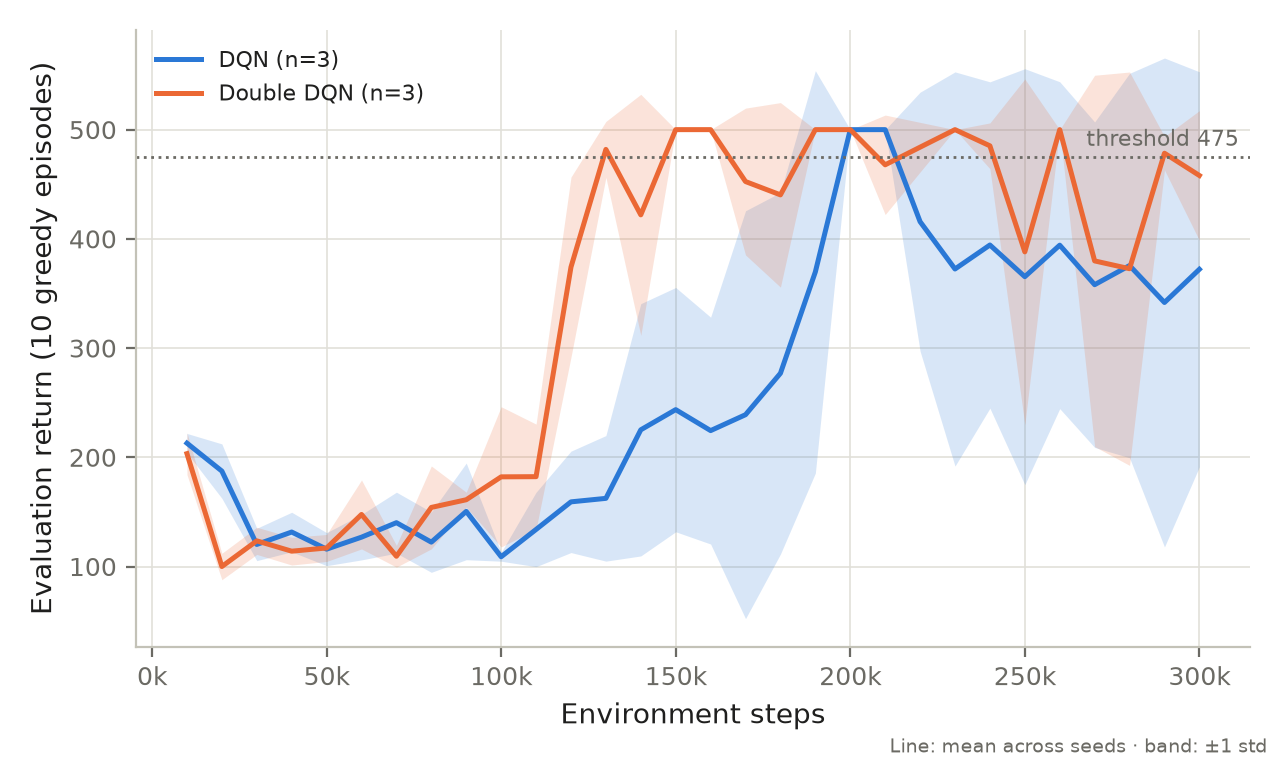
\includegraphics[width=\linewidth]{figures/tier3_cartpole_eval.png}
\caption{CartPole: evaluation return.}\end{subfigure}\hfill
\begin{subfigure}{0.33\textwidth}\centering
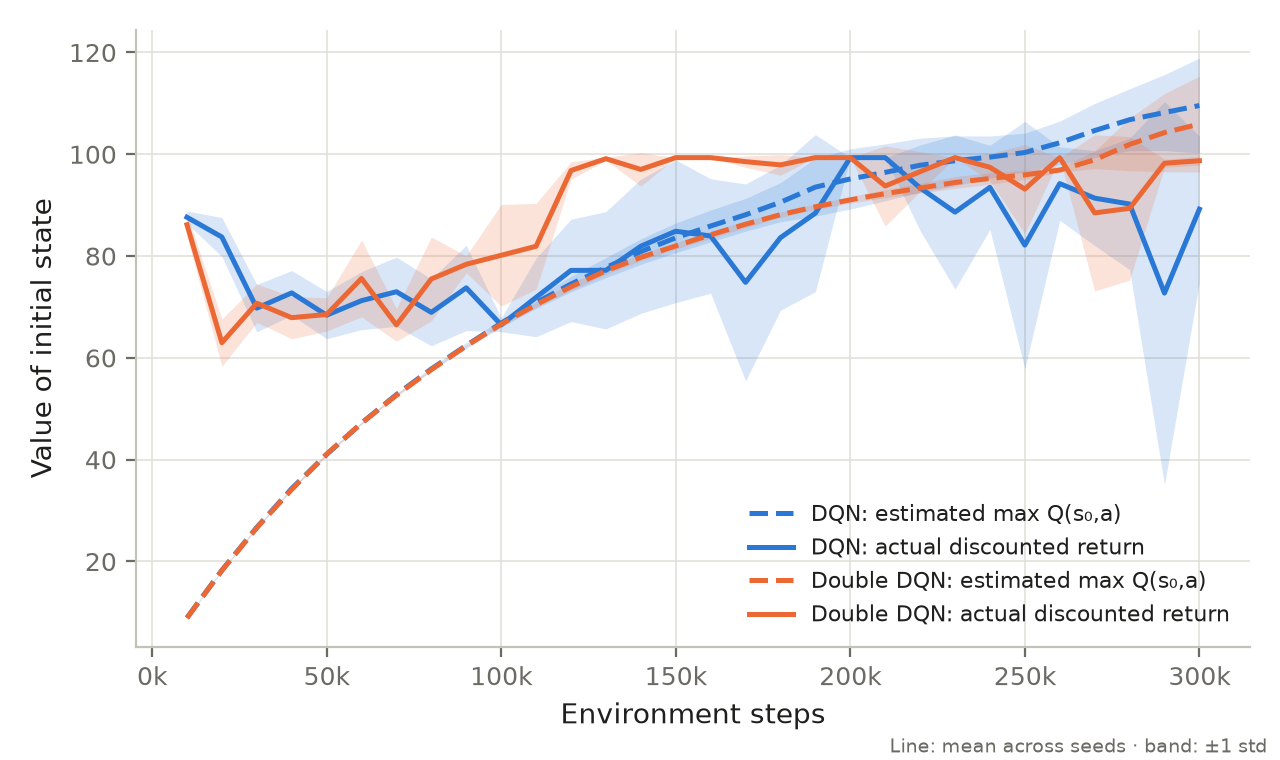
\includegraphics[width=\linewidth]{figures/tier3_cartpole_overestimation.png}
\caption{CartPole: estimated vs.\ actual $Q(s_0)$.}\end{subfigure}\hfill
\begin{subfigure}{0.33\textwidth}\centering
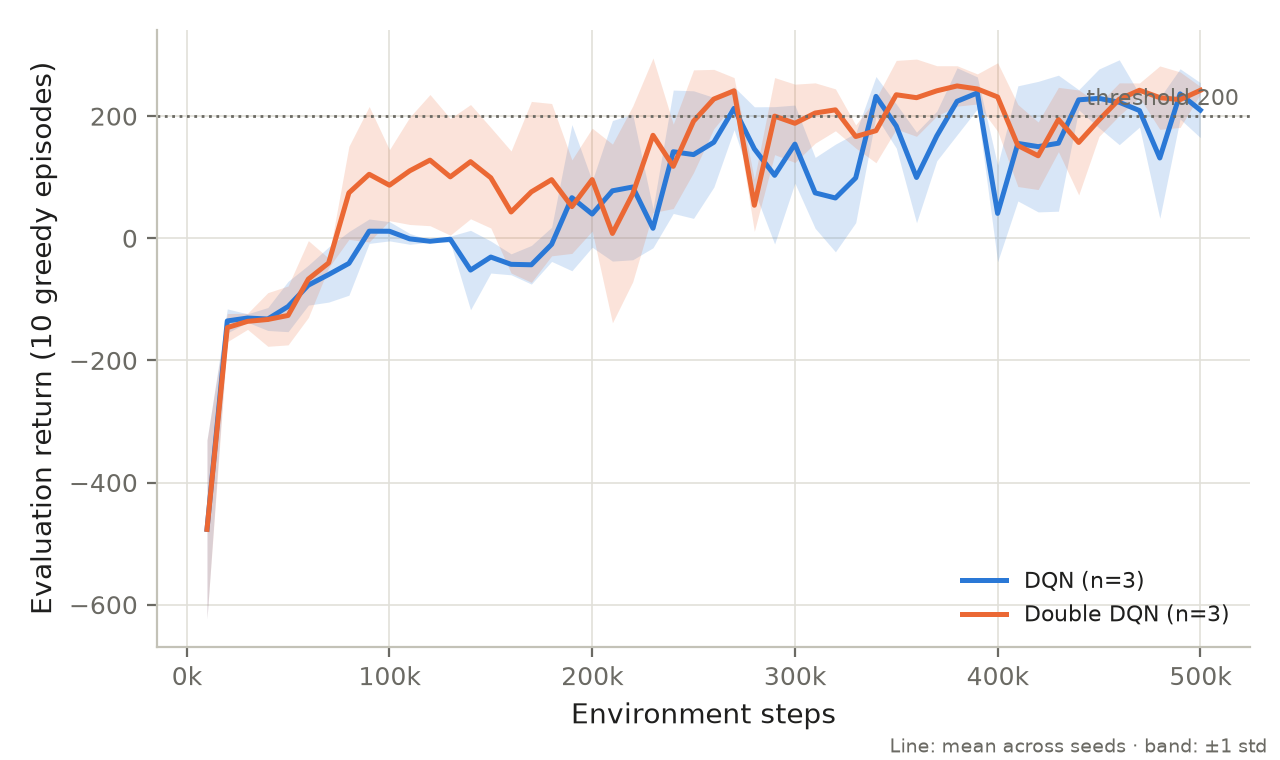
\includegraphics[width=\linewidth]{figures/tier3_eval.png}
\caption{LunarLander: evaluation return.}\end{subfigure}
\caption{Tier 3: vanilla DQN vs.\ Double DQN. In (b), dashed lines are the network's estimate $\max_a Q_\theta(s_0,a)$ and solid lines the discounted return actually obtained from $s_0$.}
\label{fig:tier3}
\end{figure*}

\begin{figure*}[t]
\centering
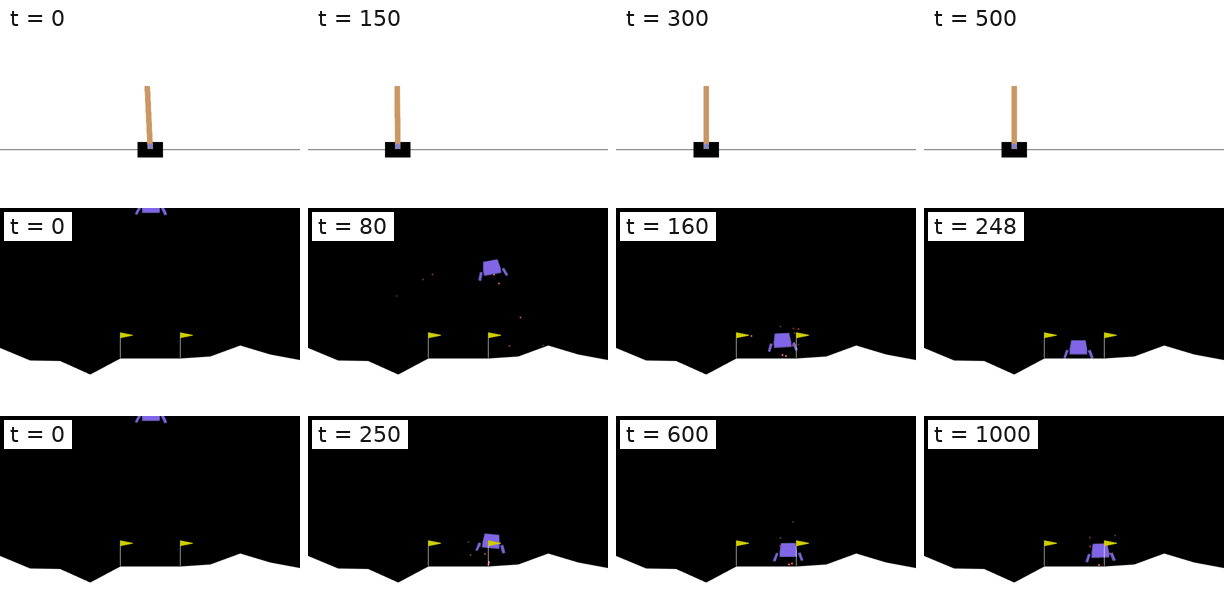
\includegraphics[width=0.82\textwidth]{figures/qualitative_frames.png}
\caption{Qualitative evidence (frames from the recorded episodes, evaluation seed 20000). Top: DQN on CartPole (seed 123) keeps the pole upright for the full 500 steps. Middle: Double DQN on LunarLander (seed 42) lands successfully (return 288.8); the episode ends at step 248 when the lander comes to rest. Bottom: DQN with learning rate $10^{-4}$ (seed 42) reaches the pad but keeps firing its engines until the 1000-step limit (return 1.9).}
\label{fig:frames}
\end{figure*}

% ==================================================================
\section{Discussion}

\textbf{Which method learned faster in Tier 1, and why?} Q-learning, in every sense we measured: it led during most of training, reached the threshold slightly earlier in environment steps, ended higher and more consistently, and ran 15 times faster. Three properties explain this. First, the problem is small: 10 bins give 10{,}000 states, which 300k steps cover well. Second, tabular updates are \emph{local}: Eq.~\eqref{eq:qlearning} changes a single entry, so improving one region of the state space cannot damage another. In DQN every gradient step moves the shared weights, and therefore the values of all states. This is the most likely mechanism behind the collapse of DQN seed 42: once the agent balances well, the buffer fills with near-upright states, transitions near failure disappear from the minibatches, and the network ``forgets'' how to recover from them (catastrophic forgetting). Third, a tabular update costs a few arithmetic operations, whereas a DQN step performs a forward and backward pass on a 128-sample batch. DQN's advantage, generalisation, only pays off when the state space is too large to tabulate, as in LunarLander.

\textbf{How sensitive was each method to its key design choice?} The tabular agent was highly sensitive to its discretisation (Table~\ref{tab:qdesign}): the number of bins changed the mean by 72 points, and placing the bins over the visited range of velocities was the single most important improvement. It also depended on the training budget, with the mean dropping from 491.1 to 444.7 between 300k and 400k steps. DQN was sensitive to its learning rate and target update period, which both control the same trade-off between speed and stability: aggressive settings (high learning rate, frequent or no target updates) learned two to three times faster but finished worse and less consistently, while conservative settings were slower and, for the lowest learning rate, could stall in a local optimum. On CartPole, the configuration with a lower learning rate and larger buffer was the difference between an agent that collapsed and one that held 500.

\textbf{What did the ablation reveal about replay and target networks?} The two components address different problems. The replay buffer decorrelates samples and spreads each transition over many updates; without it, the network is trained on a moving window of nearly identical states, overfits it, and its value estimates become badly biased (+48). It was indispensable. The target network stabilises the regression target; without it, learning was faster but the value estimate occasionally diverged and the final policy was worse. The target period study shows that this is a continuum rather than an on/off choice.

\textbf{When does Double DQN help?} Double DQN corrects the maximisation bias, so its benefit should scale with the amount of bias. Our results are consistent with this: on CartPole, where vanilla DQN overestimated the initial value beyond its theoretical maximum, Double DQN learned faster and was more stable; on LunarLander, where overestimation was small and transient, it changed little. The two-action, constant-reward structure of CartPole makes the actions' values nearly equal, which is exactly where taking a maximum over noisy estimates is most biased.

\textbf{Limitations.} With three seeds and per-episode standard deviations of 60--100 points on LunarLander, differences of 10--30 points are not conclusive; only the large effects (no replay, low learning rate, the target-period trend, the CartPole collapse) are robust. The 300k-step budget of Q-learning was selected after observing results on the same seeds used for reporting; on three independent validation seeds (7, 21, 99) the same configuration scored $486.9\pm10.4$ with 2/3 seeds solved, which is the less biased estimate. DQN hyperparameters were compared on separate seeds, but a single initial run on two reporting seeds motivated the search. Steps-to-threshold is measured on 10-episode evaluations and is noisy. Finally, LunarLander wall-clock times were measured under concurrent execution.

% ==================================================================
\section{Analysis-Only Component}

\textbf{Why locomotion tasks are unsuitable.} BipedalWalker and the MuJoCo locomotion tasks~\cite{todorov2012} have continuous, multi-dimensional actions and high-dimensional observations (Table~\ref{tab:analysis}). DQN requires a finite action set, so the torques must be discretised. With $k$ bins per joint the joint action space has $k^{m}$ elements: for HalfCheetah ($m=6$), 11 bins give $1.8\times10^6$ actions and for Ant ($m=8$) $2.1\times10^8$. The output layer would need one unit per action, the $\arg\max$ and exploration over that set become intractable, and almost every action would be tried too rarely to estimate its value; with few bins (e.g.\ 3), control becomes too coarse for smooth gaits. Tabular methods fail even earlier, on the \emph{state} side: 10 bins on BipedalWalker's 24 observations give $10^{24}$ states, and Ant's 105 observations give $10^{105}$.

\textbf{Suitable algorithm families.} These tasks call for policy-gradient and actor--critic methods that output continuous actions directly, for example as the mean and variance of a Gaussian. PPO~\cite{schulman2017} is an on-policy method whose clipped objective gives stable updates and parallelises well across environments. SAC~\cite{haarnoja2018} and TD3~\cite{fujimoto2018} are off-policy, reuse a replay buffer and are therefore more sample-efficient; SAC adds entropy maximisation for robust exploration. TD3 is directly related to our Tier 3 finding: it fights overestimation in the critic by taking the minimum of two Q-networks, the actor--critic analogue of Double DQN.

\textbf{Why tabular methods fail on pixels.} An Atari frame in ALE~\cite{bellemare2013} has $210\times160\times3$ 8-bit values, i.e.\ $256^{100{,}800}\approx10^{242{,}751}$ possible observations. Even after the usual preprocessing ($84\times84$ grey-scale), almost every observation is new, so a table would never see the same state twice and could not generalise between nearly identical frames. Moreover, a single frame is not Markov: it shows the position of the ball but not its velocity, which is why DQN stacks the last four frames and uses a convolutional network to share structure across states~\cite{mnih2015}.

\begin{table}[t]
\centering
\caption{Observation and action dimensions (verified with Gymnasium~1.4 and MuJoCo~3) and the size of the discretised action space with $k$ bins per action dimension.}
\label{tab:analysis}
\small
\setlength{\tabcolsep}{3.5pt}
\resizebox{\columnwidth}{!}{%
\begin{tabular}{@{}lcccc@{}}
\toprule
Environment & Obs. dim & Act. dim & $k=5$ & $k=11$ \\
\midrule
BipedalWalker-v3 & 24  & 4 cont.  & 625 & 14{,}641 \\
Hopper-v5        & 11  & 3 cont.  & 125 & 1{,}331 \\
HalfCheetah-v5   & 17  & 6 cont.  & 15{,}625 & $1.8\times10^6$ \\
Ant-v5           & 105$^\dagger$ & 8 cont. & $3.9\times10^5$ & $2.1\times10^8$ \\
Humanoid-v5      & 348 & 17 cont. & $7.6\times10^{11}$ & $5.1\times10^{17}$ \\
\midrule
ALE/Pong-v5      & $210{\times}160{\times}3$ & 6 disc. & \multicolumn{2}{c}{(already discrete)} \\
\bottomrule
\end{tabular}}
\vspace{2pt}

\footnotesize $^\dagger$27 if contact forces are excluded from the observation.
\end{table}

% ==================================================================
\section{Conclusion}

On a small problem, a well-discretised table beat DQN in final return, consistency and cost, because its updates are local and cannot be undone by generalisation. DQN's strength appeared on LunarLander, where tabulation is impossible and DQN solved the task in every seed. Its stability depends above all on the replay buffer, and on the target network and learning rate, which trade learning speed for reliability. Double DQN is a targeted fix: it helped where vanilla DQN overestimated values (CartPole) and was neutral where it did not (LunarLander). With more time, we would use more seeds, select the tabular budget on held-out seeds, and test whether Double DQN combined with a smaller learning rate prevents the CartPole collapse altogether.

% ==================================================================
\section*{Reproducibility}
All agents are implemented in plain Python and PyTorch, without ready-made RL agents. The repository (\url{https://github.com/adrianasofiaespinoza/proyecto_agentesinteligentes}) contains the source, JSON configurations, per-run training and evaluation logs (CSV files), trained weights and GIFs, and its README gives one command per experiment and figure.

\section*{AI-Use Statement}
Generative AI was used under the course policy. Claude (Anthropic) was used by A.~Espinoza to implement the DQN agent and its variants, the experiment, plotting and GIF scripts, to reproduce the Q-learning runs with the shared protocol, to diagnose results (e.g.\ the time-limit behaviour of the $\text{lr}=10^{-4}$ agent). T.~Chilca\~{n}an used ChatGPT (OpenAI) to support the implementation, debugging and analysis of the tabular Q-learning agent. All reported numbers were produced by our own runs and checked against the logs; environment dimensions were verified by instantiating each environment; references were checked against the original publications. Both authors reviewed all code and can explain it.

\small
\begin{thebibliography}{99}\setlength{\itemsep}{0pt}
\bibitem{bellemare2013} M.~G. Bellemare, Y.~Naddaf, J.~Veness, and M.~Bowling, ``The Arcade Learning Environment: An evaluation platform for general agents,'' \emph{J. Artificial Intelligence Research}, vol.~47, pp.~253--279, 2013.
\bibitem{fujimoto2018} S.~Fujimoto, H.~van Hoof, and D.~Meger, ``Addressing function approximation error in actor-critic methods,'' in \emph{Proc. ICML}, 2018.
\bibitem{haarnoja2018} T.~Haarnoja, A.~Zhou, P.~Abbeel, and S.~Levine, ``Soft actor-critic: Off-policy maximum entropy deep reinforcement learning with a stochastic actor,'' in \emph{Proc. ICML}, 2018.
\bibitem{lin1992} L.-J. Lin, ``Self-improving reactive agents based on reinforcement learning, planning and teaching,'' \emph{Machine Learning}, vol.~8, pp.~293--321, 1992.
\bibitem{mnih2015} V.~Mnih \emph{et al.}, ``Human-level control through deep reinforcement learning,'' \emph{Nature}, vol.~518, pp.~529--533, 2015.
\bibitem{schulman2017} J.~Schulman, F.~Wolski, P.~Dhariwal, A.~Radford, and O.~Klimov, ``Proximal policy optimization algorithms,'' arXiv:1707.06347, 2017.
\bibitem{sutton2018} R.~S. Sutton and A.~G. Barto, \emph{Reinforcement Learning: An Introduction}, 2nd~ed. MIT Press, 2018.
\bibitem{thrun1993} S.~Thrun and A.~Schwartz, ``Issues in using function approximation for reinforcement learning,'' in \emph{Proc. Connectionist Models Summer School}, 1993.
\bibitem{todorov2012} E.~Todorov, T.~Erez, and Y.~Tassa, ``MuJoCo: A physics engine for model-based control,'' in \emph{Proc. IEEE/RSJ IROS}, 2012, pp.~5026--5033.
\bibitem{towers2024} M.~Towers \emph{et al.}, ``Gymnasium: A standard interface for reinforcement learning environments,'' arXiv:2407.17032, 2024.
\bibitem{vanhasselt2016} H.~van Hasselt, A.~Guez, and D.~Silver, ``Deep reinforcement learning with double Q-learning,'' in \emph{Proc. AAAI}, 2016.
\bibitem{watkins1992} C.~J. C.~H. Watkins and P.~Dayan, ``Q-learning,'' \emph{Machine Learning}, vol.~8, pp.~279--292, 1992.
\end{thebibliography}
\normalsize

% ==================================================================
\appendix
\section{Additional Figures}
Fig.~\ref{fig:appendix} shows additional diagnostics on LunarLander-v3 referenced in Section~5 (mean over 3 seeds, band $\pm1$ std).

\begin{figure}[h]
\centering
\begin{subfigure}{\columnwidth}\centering
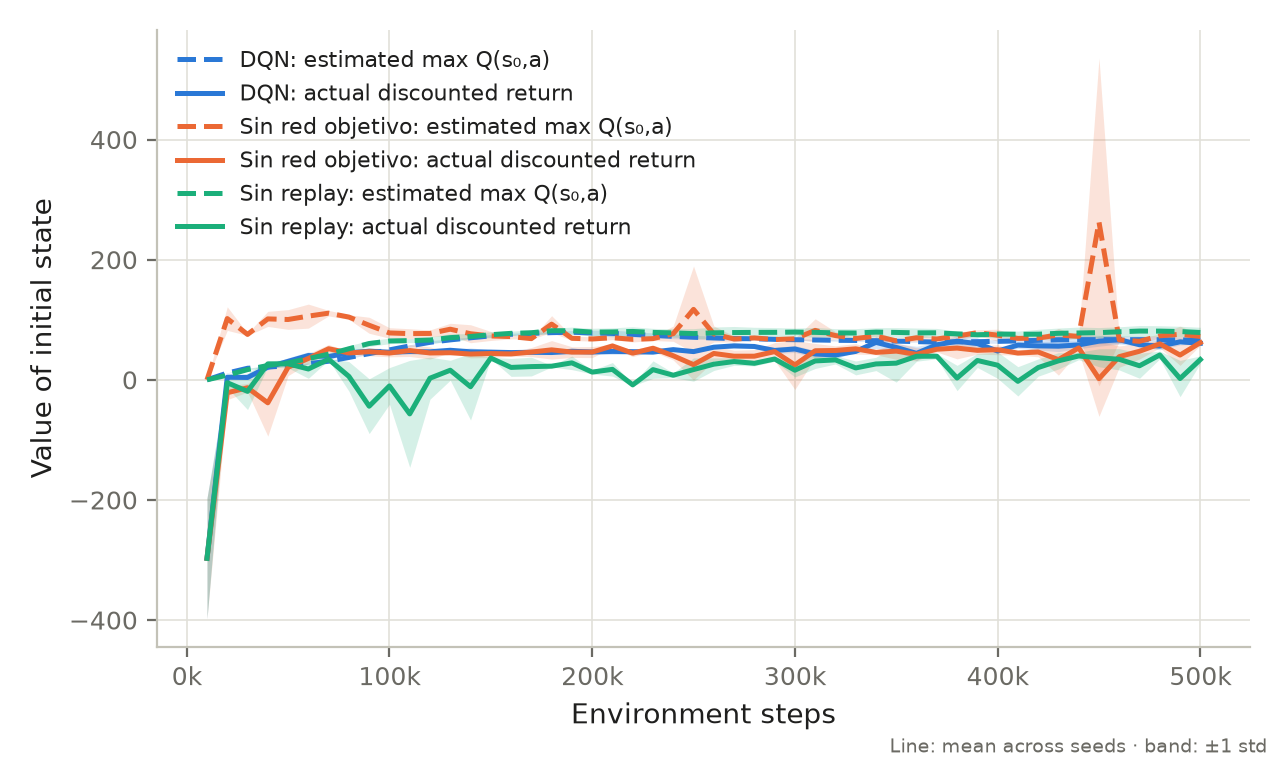
\includegraphics[width=0.92\linewidth]{figures/tier2_ablation_overestimation.png}
\caption{Tier 2 ablations: estimated (dashed) vs.\ actual (solid) $Q(s_0)$.}\end{subfigure}\\[3pt]
\begin{subfigure}{\columnwidth}\centering
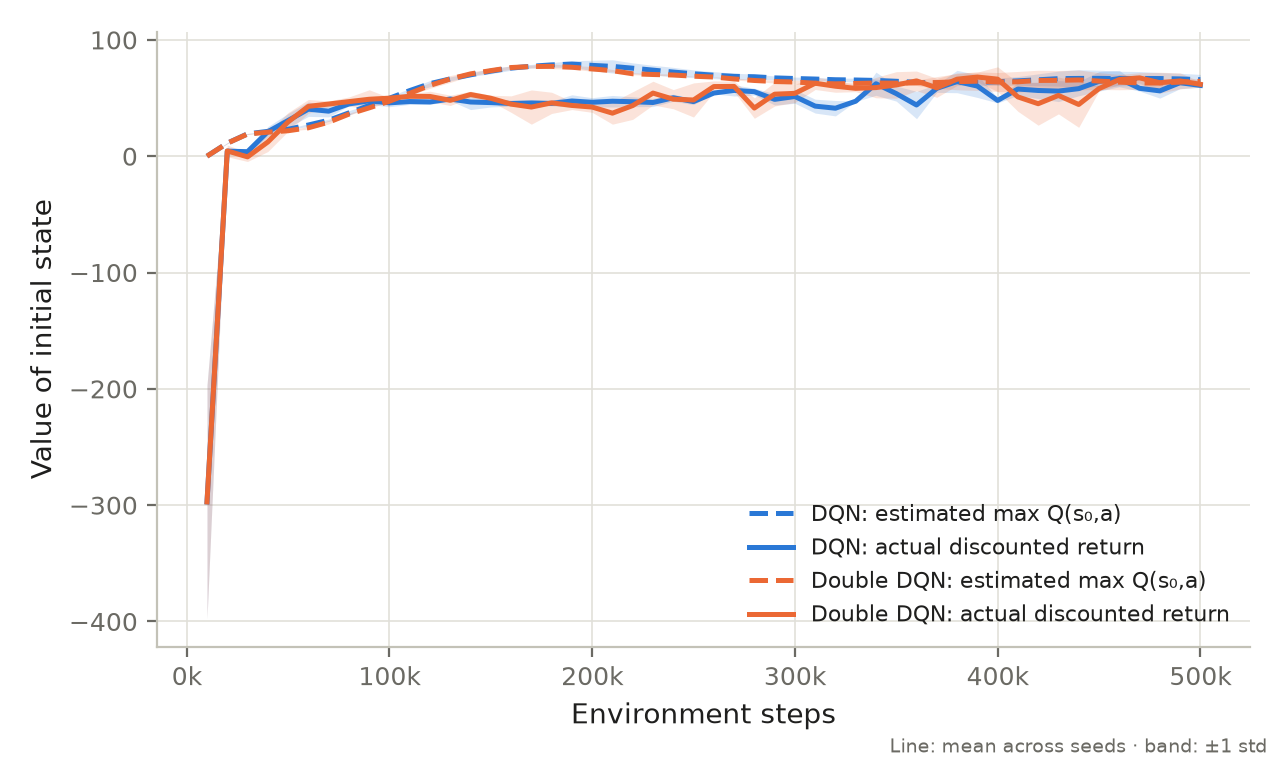
\includegraphics[width=0.92\linewidth]{figures/tier3_overestimation.png}
\caption{DQN vs.\ Double DQN: estimated (dashed) vs.\ actual (solid) $Q(s_0)$.}\end{subfigure}\\[3pt]
\begin{subfigure}{\columnwidth}\centering
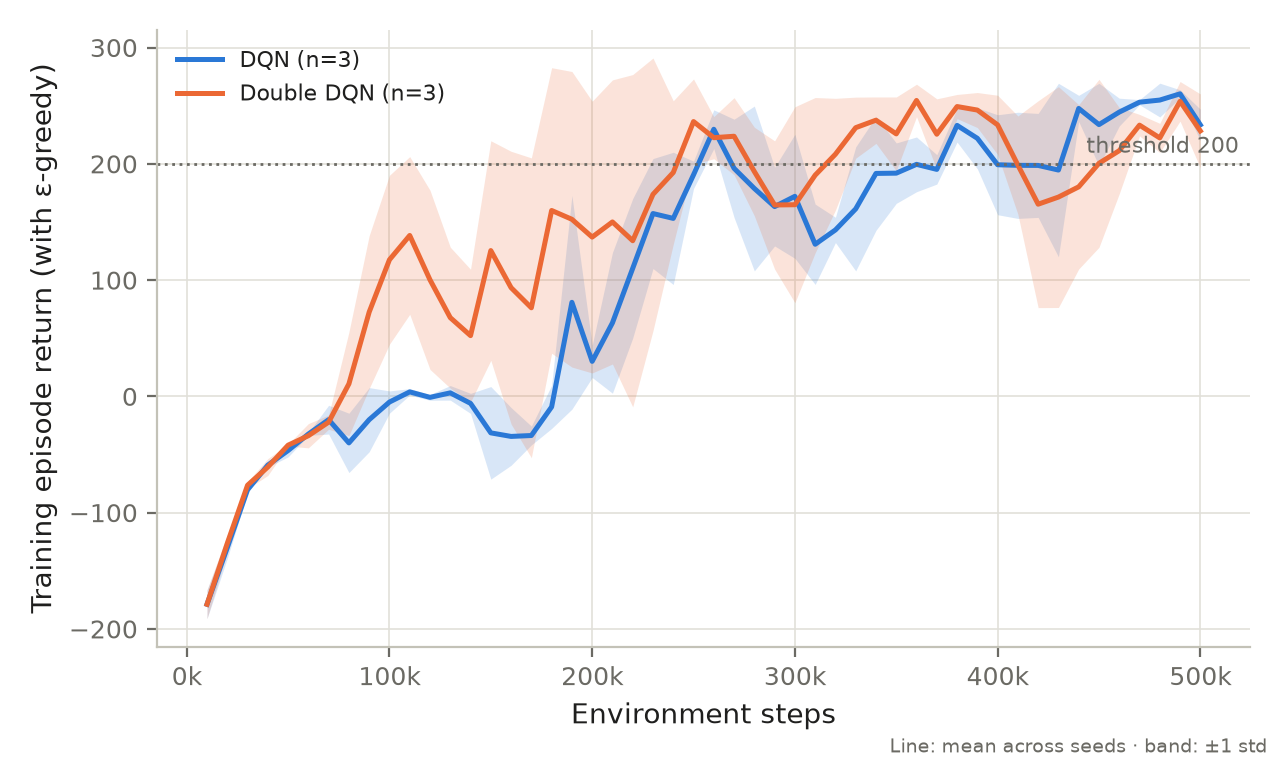
\includegraphics[width=0.92\linewidth]{figures/tier3_train.png}
\caption{DQN vs.\ Double DQN: training return (with $\eps$-greedy exploration).}\end{subfigure}
\caption{Additional diagnostics on LunarLander-v3.}
\label{fig:appendix}
\end{figure}

\end{document}
